%%%%%%%%%%%%%%%%%%%%%%%%%%%%%%%%%%%%%%%%%%%%%%%%%%%%%%%%%%%%
% RESULTS
%%%%%%%%%%%%%%%%%%%%%%%%%%%%%%%%%%%%%%%%%%%%%%%%%%%%%%%%%%%%
\section{Experiments}


\subsection{PDE Problem Settings}
\label{sec:exp-forward-inverse}

We show the usefulness of DiffusionPDE across various PDEs for inverse and forward problems and compare it against recent learning-based techniques. We test on the following families of PDEs.

\vspace{-1em}\paragraph{Darcy Flow.} Darcy flow describes the movement of fluid through a porous medium. In our experiment, we consider the static Darcy Flow with a no-slip boundary $\partial\Omega$
\begin{equation}
    \begin{aligned}
        -\nabla\cdot(\a(\c)\nabla \u(\c))&=q(\c),\quad && \c\in\Omega \\
        \u(\c)&=0, && \c\in\partial\Omega
    \end{aligned}
\end{equation}
Here the coefficient $\a$ has binary values. We set $q(\c) = 1$ for constant force. The PDE guidance function is thus $f=\nabla\cdot(\a(\c)\nabla \u(\c))+q(\c)$.

\vspace{-1em}
\paragraph{Inhomogeneous Helmholtz Equation.} We consider the static inhomogeneous Helmholtz Equation with a no-slip boundary on $\partial\Omega$, which describes wave propagation:
\begin{equation}\label{eq:inhomogeneous-helmholtz}
    \begin{aligned}
        \nabla^2\u(\c)+k^2\u(\c)&=\a(\c),\quad && \c\in\Omega \\
        \u(\c)&=0, && \c\in\partial\Omega
    \end{aligned}
\end{equation}
The coefficient $\a$ is a piecewise constant function and $k$ is a constant. Note \ref{eq:inhomogeneous-helmholtz} is the Poisson equation when $k=0$. 
Setting $k=1$ for Helmholtz equations, the PDE guidance function is $f = \nabla^2\u(\c)+k^2\u(\c)-\a(\c)$. 


\vspace{-1em}\paragraph{Non-bounded Navier-Stokes Equation.} We study the non-bounded incompressive Navier-Stokes equation regarding the vorticity. 
\begin{equation}
    \begin{aligned}
        \begin{aligned}
            \partial_tw(\c, \t)+v(\c, \t)\cdot\nabla w(\c, \t)
        \end{aligned} & 
        \begin{aligned} 
            =\nu\Delta w(\c, \t)+q(\c),
        \end{aligned} && \c\in\Omega, \t\in(0,T] \\
        \begin{aligned}
            \nabla\cdot v(\c, \t)
        \end{aligned}
        & =0, && \c\in\Omega, \t\in[0,T] 
    \end{aligned}
\end{equation}
Here $w=\nabla\times v$ is the vorticity, $v(\c, \t)$ is the velocity at $\c$ at time $\t$, and  $q(\c)$ is a force field. We set the viscosity coefficient $\nu=10^{-3}$ and correspondingly the Reynolds number $Re=\frac{1}{\nu}=1000$. 

DiffusionPDE learns the joint distribution of $w_0$ and $w_T$ and we take $T=10$ which simulates $1$ second. Since $T\gg0,$ we cannot accurately compute the PDE loss from our model outputs. Therefore, given that $\nabla\cdot w(\c, \t)=\nabla\cdot(\nabla\times v)=0$, we use simplified $f=\nabla\cdot w(\c, \t)$. 
% \jj{the divergence term requires you  partial w / partial tau, which we don't have?}

\vspace{-1em}
\paragraph{Bounded Navier-Stokes Equation.} We study the bounded 2D imcompressive Navier Stokes regarding the velocity $v$ and pressure $p$. 
\begin{equation}
    \begin{aligned}
        \partial_tv(\c, \t)+v(\c, \t)\cdot\nabla v(\c, \t)+\frac{1}{\rho}\nabla p&=\nu\nabla^2v(\c, \t), \quad && \c\in\Omega, \t\in(0,T] \\
        \nabla\cdot v(\c, \t) &=0, && \c\in\Omega, \t\in(0,T].
    \end{aligned}
\end{equation}
We set the viscosity coefficient $\nu=0.001$ and the fluid density $\rho=1.0$. We generate 2D cylinders of random radius at random positions inside the grid. Random turbulence flows in from the top of the grid, with the velocity field satisfying no-slip boundary conditions at the left and right edges, as well as around the cylinder $\partial \Omega_{left, right, cylinder}$. DiffusionPDE learns the joint distribution of $v_0$ and $v_T$ at $T=4$, which simulates $0.4$ seconds. Therefore, we similarly use $f=\nabla\cdot v(\c, \t)$ as before.


\vspace{-1em}
\paragraph{Burgers' Equation.} We study the Burgers' equation with periodic boundary conditions on a 1D spatial domain of unit length $\Omega=(0, 1)$. We set the viscosity to $\nu=0.01$. In our experiment, the initial condition $u_0$ has a shape of $128\times 1$, and we take 127 more time steps after the initial state to form a 2D $u_{0:T}$ of size $128\times 128$.
\begin{equation}
    \begin{aligned}\partial_tu(\c, \t)+\partial_{\c}(u^2(\c, \t)/2)&=\nu\partial_{\c\c}u(\c, \t),\quad &&\c\in\Omega,\t\in(0,T]\\u(\c,0)&=u_0(\c),&&\c\in\Omega\end{aligned}
\end{equation}
We can reliably compute  $f=\partial_tu(\c, \t)+\partial_{\c}(u^2(\c, \t)/2)-\nu\partial_{\c\c}u(\c, \t)$ with finite difference since we model densely on the time dimension.

\vspace{-0.5em}
\subsection{Dataset Preparation and  Training}\label{sec:preparation}

We first test DiffusionPDE on jointly learning the forward mapping $\mathcal{F}: \A\to\U$ and the inverse mapping $\mathcal{I}: \U\to\A$ given sparse observations. In our experiments, we define our PDE over the unit square $\Omega = (0,1)^2$, which we represent as a $128\times 128$ grid. We utilize Finite Element Methods (FEM) to generate our training data. Specifically, we run FNO's \cite{li2020fourier} released scripts to generate Darcy Flows and the vorticities of the Navier-Stokes equation. Similarly, we generate the dataset of Poisson and Helmholtz using second-order finite difference schemes. To add more complex boundary conditions, we use Difftaichi \cite{hu2019difftaichi} to generate the velocities of the bounded Navier-Stokes equation. We train the joint diffusion model for each PDE on three A40 GPUs for approximately 4 hours, using 50,000 data pairs. For Burgers' equation, we train the diffusion model on a dataset of 50,000 samples produced as outlined in FNO \cite{li2020fourier}. We randomly select 5 out of 128 spatial points on $\Omega$ to simulate sensors that provide measurements across time.



\vspace{-0.4em}
\subsection{Baseline Methods}
\vspace{-0.3em}
We compare DiffusionPDE with state-of-the-art learning-based methods, including PINO \cite{li2021physics}, DeepONet \cite{lu2021learning}, PINNs \cite{raissi2019physics}, and FNO \cite{li2020fourier}. However, note that none of these methods show operation on partial observations. These methods can learn mappings between $\a$ and $\u$ or $\u_0$ and $\u_{1:T}$ with full observations, allowing them to also solve the mapping between $\u_0$ and $\u_T$. PINNs map input $\a$ to output $\u$ by optimizing a combined loss function that incorporates both the solution $\u$ and the PDE residuals. DeepONet employs a branch network to encode input function values sampled at discrete points and a trunk network to handle the coordinates of the evaluated outputs. FNO maps from the parametric space to the solution space using Fourier transforms. PINO enhances FNO by integrating PDE loss during training and refining the model with PDE loss finetuning. We train all four baseline methods on both forward and inverse mappings using full observation of $\a$ or $\u$ for both static and dynamic PDEs. We tried training the baseline models on partial observations, but we noticed degenerate training outcomes (see supplementary for details). Overall, they are intended for {\em full observations} and may not be suitable for sparse measurements. 

More closely related to our method, GraphPDE~\cite{zhao2022learning} demonstrates the ability to recover the initial state using sparse observations on the final state, a task that other baselines struggle with. Therefore, we compare against GraphPDE for the inverse problem of bounded Navier-Stokes (NS) equation, which is the setup used in their report. GraphPDE uses a trained latent space model and a bounded forward GNN model to solve the inverse problem with sparse sensors and thus is incompatible with unbounded Navier-Stokes. We create bounded meshes using our bounded grids to train the GNN model and train the latent prior with $v_{0:T}$ for GraphPDE.


\begin{table}[t!]
    \caption{Relative errors of solutions (or final states) and coefficients (or initial states) when solving forward and inverse problems respectively with sparse observations. Error rates are used for the inverse problem of Darcy Flow.}
    \label{table:merged_results}
    \centering
    \begin{tabular}{p{2cm}lccccc}
        \toprule
        & & DiffusionPDE & PINO & DeepONet & PINNs & FNO \\
        \midrule
        \multirow{2}{*}{Darcy Flow} & Forward & \textbf{2.5\%} & 35.2\% & 38.3\% & 48.8\% & 28.2\% \\
        & Inverse & \textbf{3.2\%} & 49.2\% & 41.1\% & 59.7\% & 49.3\% \\
        \midrule
        \multirow{2}{*}{Poisson} & Forward & \textbf{4.5\%} & 107.1\% & 155.5\% & 128.1\% & 100.9\% \\
        & Inverse & \textbf{20.0\%} & 231.9\% & 105.8\% & 130.0\% & 232.7\% \\
        \midrule
        \multirow{2}{*}{Helmholtz} & Forward & \textbf{8.8\%} & 106.5\% & 123.1\% & 142.3\% & 98.2\% \\
        & Inverse & \textbf{22.6\%} & 216.9\% & 132.8\% & 160.0\% & 218.2\% \\
        \midrule
        \multirow{2}{2cm}{Non-bounded Navier-Stokes} & Forward & \textbf{6.9\%} & 101.4\% & 103.2\% & 142.7\% & 101.4\% \\
        & Inverse & \textbf{10.4\%} & 96.0\% & 97.2\% & 146.8\% & 96.0\% \\
        \midrule
        \multirow{2}{2cm}{Bounded Navier-Stokes} & Forward & \textbf{3.9\%} & 81.1\% & 97.7\% & 100.1\% & 82.8\% \\
        & Inverse & \textbf{2.7\%} & 69.5\% & 91.9\% & 105.5\% & 69.6\% \\
        \bottomrule
    \end{tabular}
\end{table}

% \begin{table}
%   \caption{Forward and inverse model results with sparse observation on initial and final states respectively}
%   \label{table:error_all}
%   \centering
%   \begin{tabular}{llll}
%     \toprule
%     &Burgers' Equation &\multicolumn{2}{c}{Navier-Stokes}                  \\
%     \cmidrule(r){2-4}
%     Method     & total error   & initial state error & final state error \\
%     \midrule
%     DiffusionPDE & 2.68\% & 8.4\% & 6.5\%   \\
%     PINO &  85.7\% & - & 99.5\%  \\
%     DeepONet & - & - & 103.2\% \\
%     PINNs & 92.7\% & - & 183.5\% \\
%     FNO & 90.0\% & - & 99.5\% \\
%     \bottomrule
%   \end{tabular}
% \end{table}

% \begin{table}
%   \caption{Solve static PDEs}
%   \label{table:error_all_static}
%   \centering
%   \begin{tabular}{lllllll}
%     \toprule
%     &\multicolumn{2}{c}{Darcy Flow} &\multicolumn{2}{c}{Poisson} &\multicolumn{2}{c}{Helmholtz}                  \\
%     \cmidrule(r){2-7}
%     Method     & $a$ accuracy   & $u$ error & $a$ error & $u$ error & $a$ error & $u$ error \\
%     \midrule
%     DiffusionPDE & 90.8\%  & 5.6\% & 20.0\% & 4.5\% & 22.6\% & 8.8\%   \\
%     PINO & 47.5\% & 44.9\% & 98.5\% & 107.1\%  & 98.5\% & 106.5\%      \\
%     DeepONet & - & 38.1\% & - & 155.5\% & - & 123.1\% \\
%     PINNs & - & 162.3\% & - & 173.6\% & - & 153.2\% \\
%     FNO & - & 25.5\% & - & 100.9\% & - & 98.2\% \\
%     \bottomrule
%   \end{tabular}
% \end{table}

While we employ guided sampling to reconstruct the solutions, Classifier-Free Guidance (CFG) \cite{ho2022classifier} offers an alternative approach where the diffusion model is conditioned on sparse input data. Shu et al. \cite{shu2023physics} extend this method by developing an optimized CFG approach that conditions on the PDE loss, using the observation as a low-resolution input. Additionally, OFormer \cite{li2022transformer} is another model designed to reconstruct the full solution using transformers, offering a shorter inference runtime. Consequently, we compare our approach against these methods for solving the unbounded Navier-Stokes equation.


\vspace{-0.5em}
\subsection{Main Evaluation Results}
\vspace{-0.3em}

\begin{figure}[t!]
    \centering
    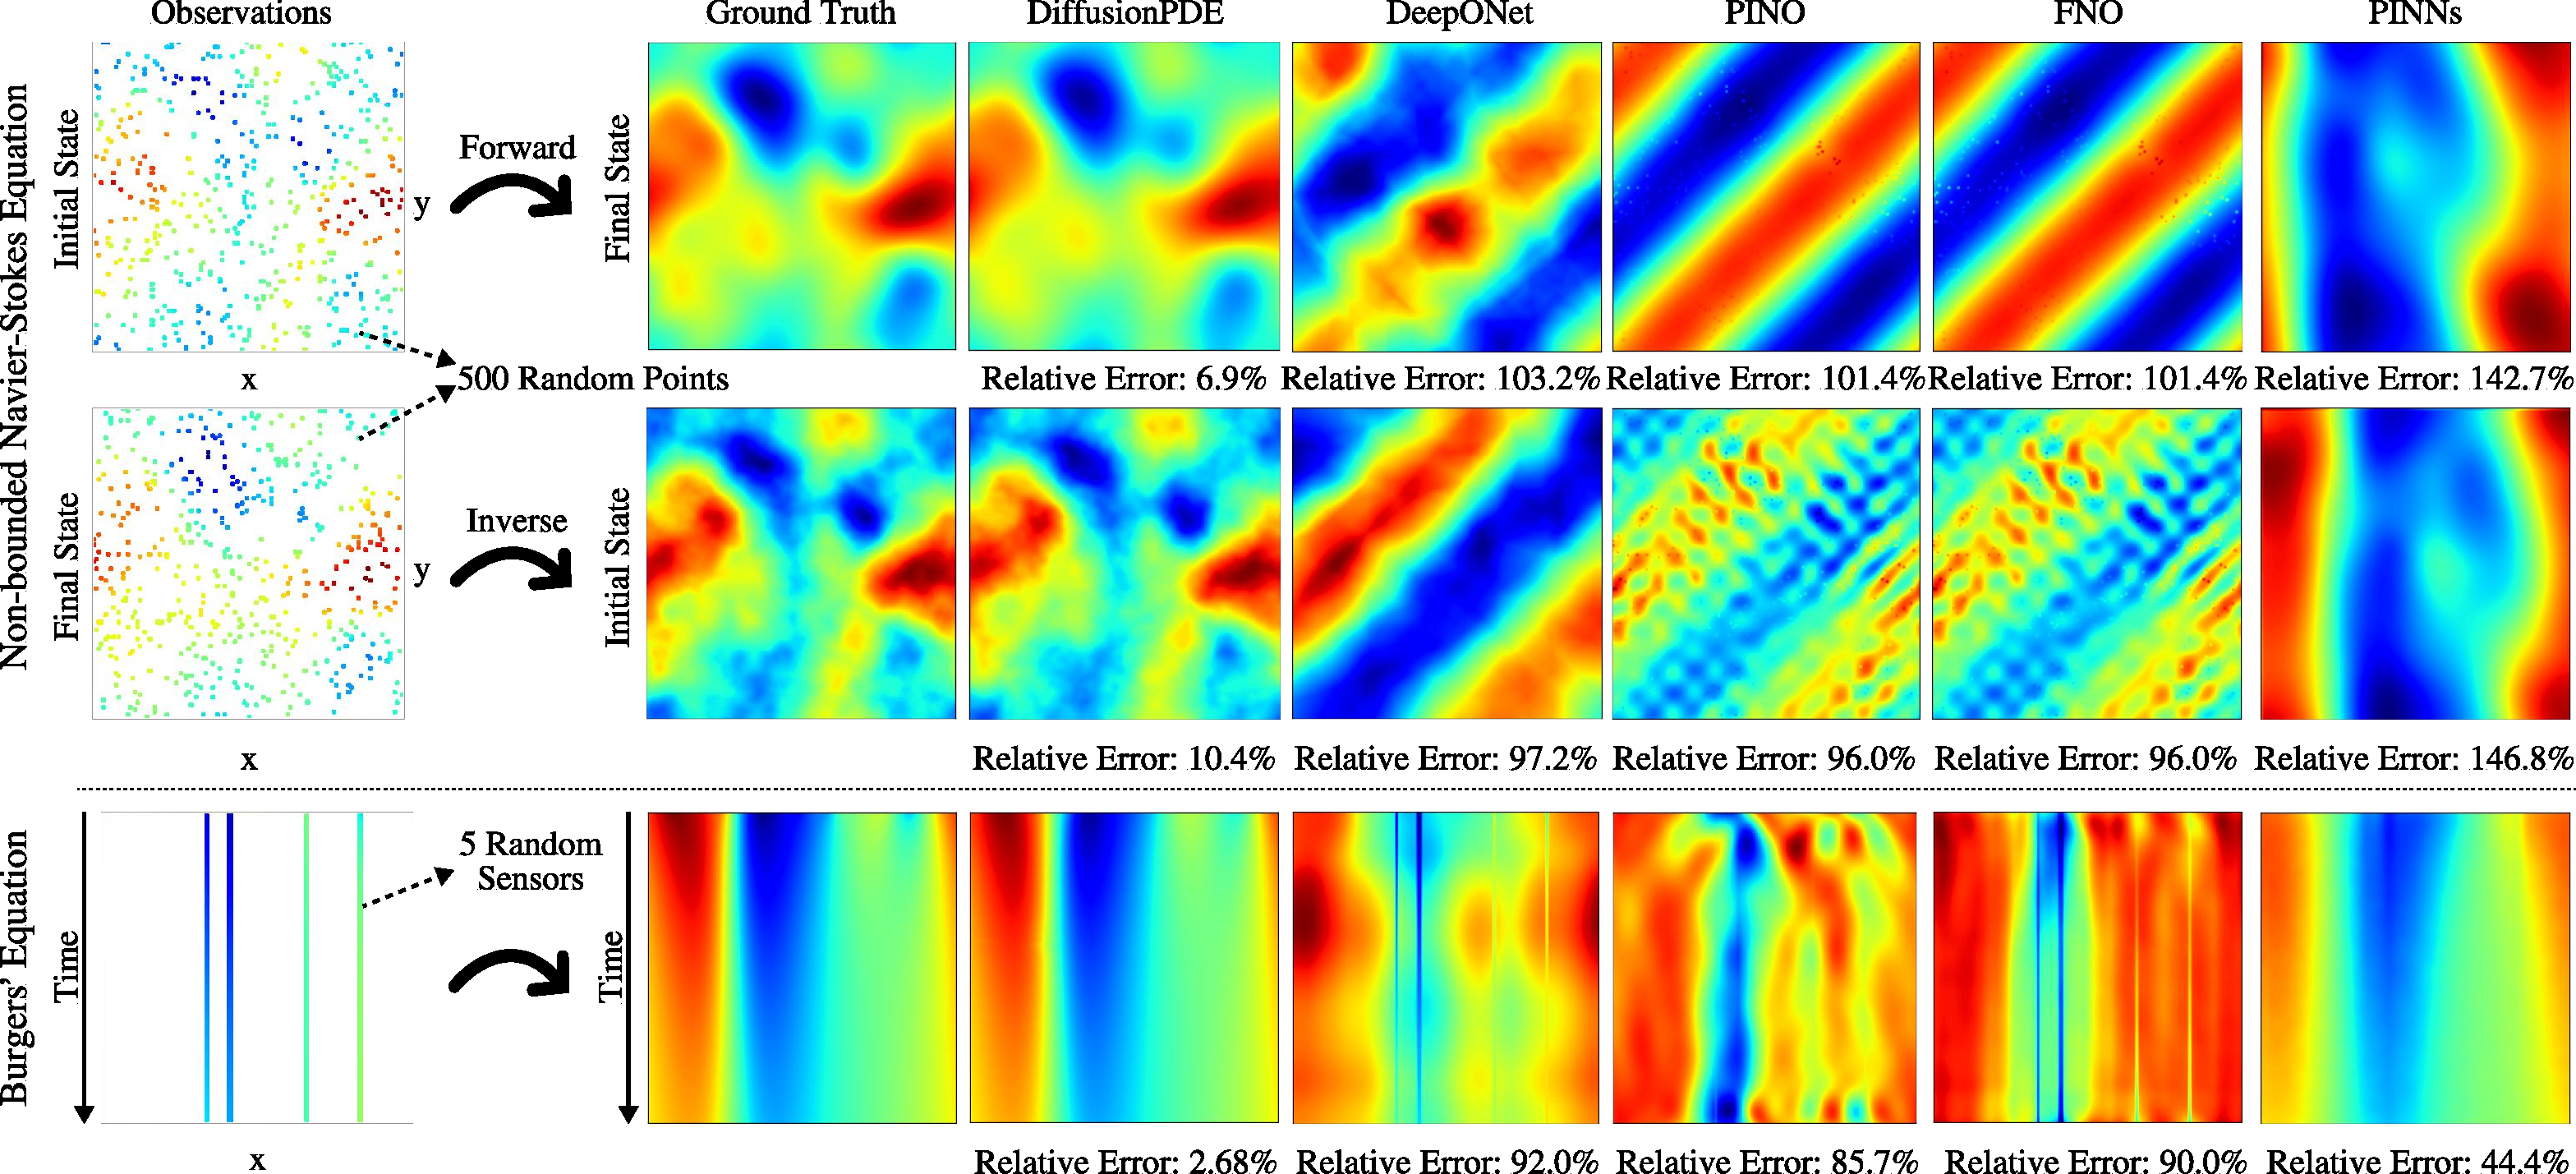
\includegraphics[width=0.99\textwidth]
    {figs/main_ns_and_burgers_updated.pdf}
    \caption{We compare DiffusionPDE with state-of-the-art neural PDE solvers \cite{li2020fourier, li2021physics, lu2021learning, raissi2019physics}. In the forward Navier-Stokes problem, we give $500$ sparse observations of the initial state to solve for the final state. In the inverse set-up, we take observations of the final state and solve for the initial. 
    For the Burgers' equation, we use $5$ sensors throughout all time steps and want to recover the solution at all time steps. Note that we train on neighboring snapshot pairs for the baselines in order to add continuous observations of the Burgers' equation. Results show that existing methods do not support PDE solving under sparse observations, and we believe they are not easily extendable to do so. We refer readers to the supplementary for a complete set of visual results.
   }\vspace{-1em}
    \label{fig:nonbounded_ns_all}
\end{figure}


We respectively address the forward problem and the inverse problem with sparse observations of $\a$ or $\u$. For the forward problem, we randomly select coefficients (initial states) as sparse observations and then compare the predicted solutions (final states) with the ground truth. Specifically, we select $500$ out of $128\times 128$ points, approximately $3\%$, on the coefficients of Darcy Flow, Poisson equation, Helmholtz equation, and the initial state of the non-bounded Navier-Stokes equation. For the bounded Navier-Stokes equation, we use $1\%$ observed points beside the boundary of the cylinder in 2D. Similarly, for the inverse problem, we randomly sample points on solutions (final states) as sparse observations, using the same number of observed points as in the forward model for each PDE.


We show the relative errors of all methods regarding both forward and inverse problems in Table \ref{table:merged_results}. Since the coefficients of Darcy Flow are binary, we evaluate the error rates of our prediction. Non-binary data is evaluated using mean pixel-wise relative error. We report error numbers averaged across 1,000 random scenes and observations for each PDE. DiffusionPDE outperforms other methods including PINO \cite{li2021physics}, DeepONet~\cite{lu2021learning}, PINNs~\cite{raissi2019physics}, and FNO~\cite{li2020fourier} for both directions with sparse observations, demonstrating the novelty and uniqueness of our approach. For the inverse problems of the Poisson and Helmholtz equations, DiffusionPDE exhibits higher error rates due to the insufficient constraints within the coefficient space, produced from random fields. In Fig. \ref{fig:nonbounded_ns_all}, we visualize the results for solving both the forward and inverse problem of the non-bounded Navier-Stokes. We refer to the {\em supplementary} for additional visual results. While other methods may produce partially correct results, DiffusionPDE outperforms them and can recover results very close to the ground truth. 

For the inverse problem of the bounded Navier-Stokes equation, we further compare DiffusionPDE with GraphPDE, as illustrated in Fig. \ref{fig:bounded_ns_withGraphPDE}. Our findings reveal that DiffusionPDE surpasses GraphPDE \cite{zhao2022learning} in accuracy, reducing the relative error from $12.0\%$ to $2.7\%$ with only $1\%$ observed points.


We further show whether DiffusionPDE can jointly recover both $\a$ and $\u$ by analyzing the retrieved $\a$ and $\u$ with sparse observations on different sides as well as on both sides. In Fig. \ref{fig:darcy_a_u_au}, we recover the coefficients and solutions of Darcy Flow by randomly observing $500$ points on only coefficient space, only space solution space, and both. Both coefficients and solutions can be recovered with low errors for each situation. We therefore conclude that DiffusionPDE can solve the forward problem and the inverse problem simultaneously with sparse observations at any side without retraining our network.



\begin{figure}[t]
    \centering
    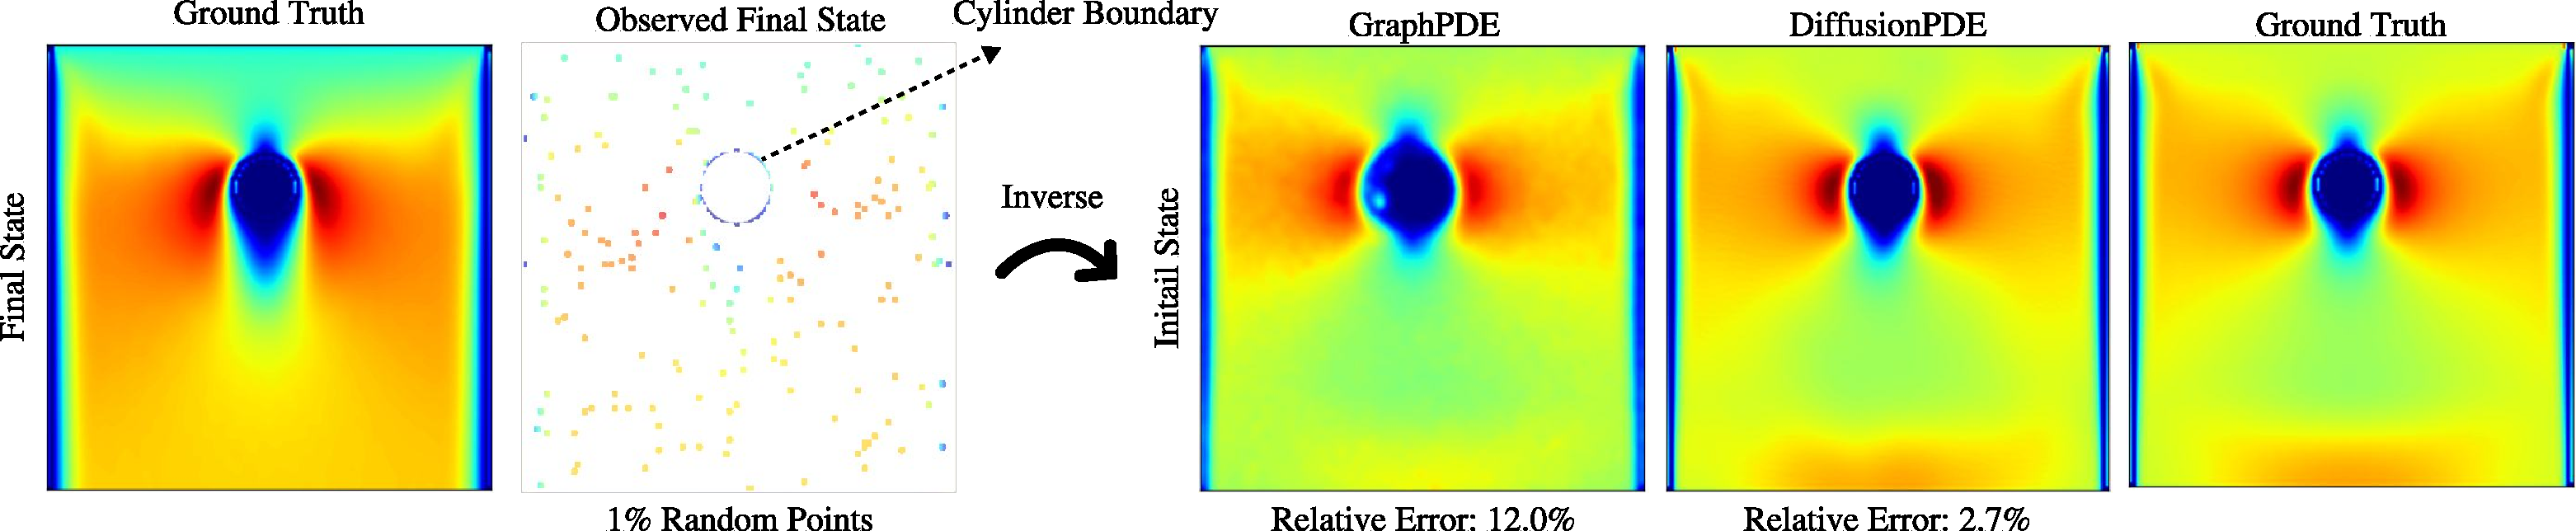
\includegraphics[width=0.99\textwidth]{figs/ns/bounded_NS_withGraphPDE.pdf}
    \caption{We compare GraphPDE \cite{zhao2022learning} and our method for solving the inverse bounded Navier-Stokes equation. Given the boundary conditions and $1\%$ observations of the final vorticity field, we solve the initial vorticity field. We set the fliuds to flow in from the top, with boundary conditions at the edges and a middle cylinder. While GraphPDE can recover the overall pattern of the initial state, it suffers from noise when the fluid passes the cylinder and misses the high vorticities at the bottom.}
    \label{fig:bounded_ns_withGraphPDE}
\end{figure}

\subsection{Advantage of Guided Sampling}

To demonstrate the clear advantage of our guided sampling method, we evaluate both the forward and inverse processes of the unbounded Navier-Stokes equation, comparing our DiffusionPDE approach with Diffusion using  CFG when considering only the initial and final states given 500 observation points, as illustrated in Fig. \ref{fig:diffusionpde-vs-diffusioncfg}. Our DiffusionPDE method consistently achieves lower relative errors across both evaluations.

Furthermore, in Fig. \ref{fig:vs-shu-and-oformer}, we compare our results with those of Shu et al. \cite{shu2023physics}, where the full time intervals are solved autoregressively using an optimized CFG method. In their approach, the error in the final state increases to approximately 13\%, which is notably higher than that of our two-state model. Additionally, the relative errors of the transformer-based approach, OFormer \cite{li2022transformer}, are around 17\% and 23\%, which are significantly larger than those observed with DiffusionPDE.


\subsection{Recovering Solutions Throughout a Time Interval}\label{sec:recover-all}

We demonstrate that DiffusionPDE is capable of retrieving all time steps throughout the time interval $[0,T]$ from continuous observations on sparse sensors. To evaluate its ability to recover $u_{0:T}$ with sparse sensors, we study the 1D dynamic Burgers' equation, where DiffusionPDE learns the distribution of $u_{0:T}$ using a 2D diffusion model. To apply continuous observation on PINO, DeepONet, FNO, and PINNs, we train them on neighboring snapshot pairs. Our experiment results in a test relative error of 2.68\%, depicted in Fig. \ref{fig:nonbounded_ns_all}, which is significantly lower than other methods. 


\subsection{Additional Analysis}\label{sec:ablation}
We examine the effects of different components of our algorithm such as PDE loss and observation samplings.
We strongly encourage readers to view the supplementary for more details of these analyses as well as additional experiments.
\paragraph{PDE Loss.} 

\vspace{-0.5em}
To verify the role of the PDE guidance loss of Eq. \ref{eq:diffusionpde-loss} during the denoising process, we visualize the errors of recovered $\a$ and $\u$ of Helmholtz equation with or without PDE loss. Here, we run our DPS algorithm with 500 sparse observed points on both the coefficient $\a$ and solution $\u$ and study the effect of the additional PDE loss guidance. The relative error of $\u$ reduces from $9.3\%$ to $0.6\%$, and the relative error of $\a$ reduces from $13.2\%$ to $9.4\%$. Therefore, we conclude that PDE guidance helps smooth the prediction and improve the accuracy.

\vspace{-0.5em}
\paragraph{Number of Observations.} We examine the results of DiffusionPDE in solving forward and inverse problems when there are $100$, $300$, $500$, and $1000$ random observations on $\a$, $\u$, or both $\a$ and $\u$. The error of DiffusionPDE decreases as the number of sparse observations increases. DiffusionPDE is capable of recovering both $\a$ and $\u$ with errors $1\% \sim 10\%$ with approximately $6\%$ observation points at any side for most PDE families. DiffusionPDE becomes insensitive to the number of observations and can solve the problems well once more than $3\%$ of the points are observed. 

\vspace{-0.5em}
\paragraph{Observation Sampling Pattern.} While CFG struggles with robustness, we show that DiffusionPDE is robust to different sampling patterns of the sparse observations, including grid and non-uniformly concentrated patterns. Note that even when conditioned on the full observations, our approach performs on par with the current best methods, likely due to the inherent resilience of our guided diffusion algorithm. Additionally, DiffusionPDE can leverage continuous coordinates with bilinear interpolation in the prediction space to obtain predicted values for points that do not lie directly on the grid, without compromising accuracy.

\begin{figure}[t]
    \centering
    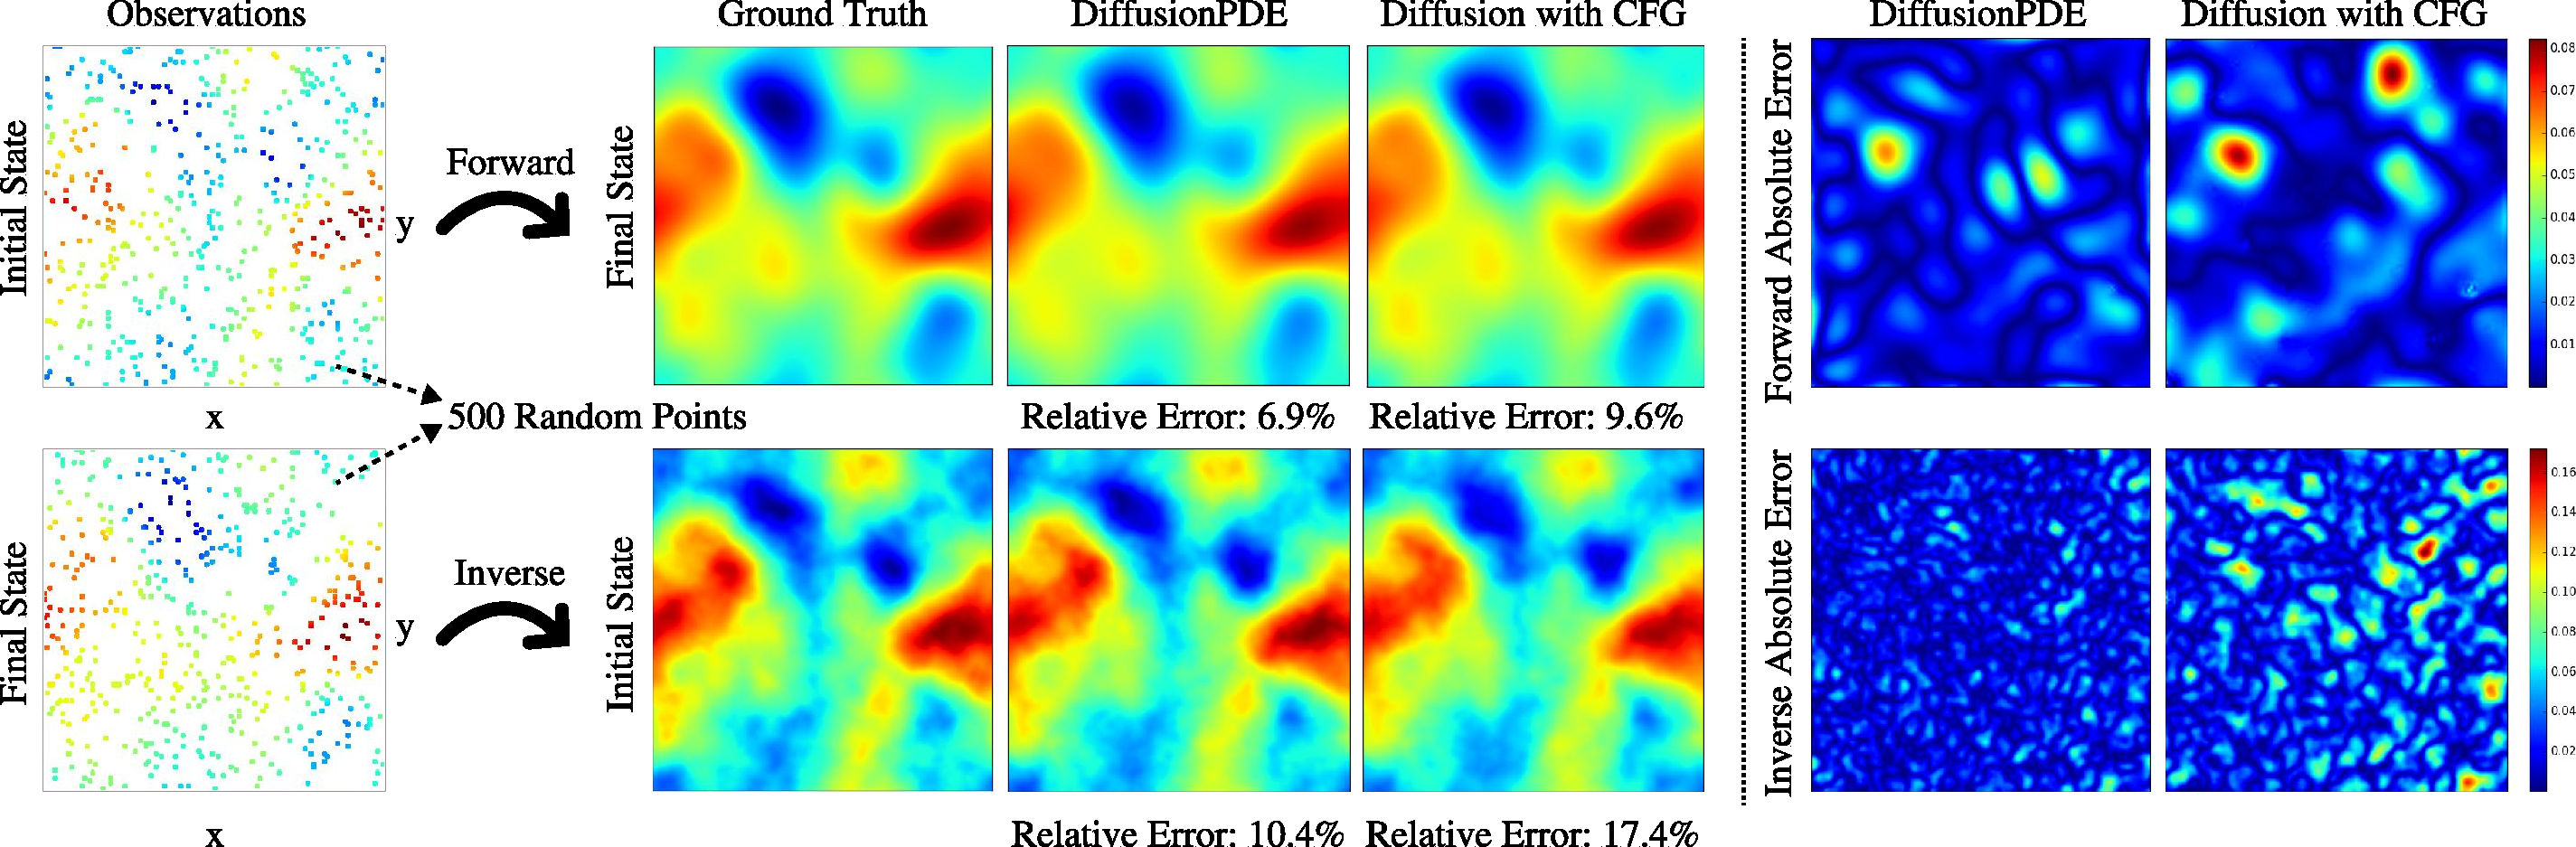
\includegraphics[width=0.99\textwidth]{figs/rebuttal/DiffusionPDE_14.pdf}
    \caption{We compare the performance of DiffusionPDE and Diffusion with CFG for the unbounded Navier-Stokes equation, and visualize the error. With 500 observation points, DiffusionPDE demonstrates superior accuracy, achieving lower errors in both forward and inverse problem-solving.}
    \label{fig:diffusionpde-vs-diffusioncfg}
\end{figure}

\begin{figure}[t]
    \centering
    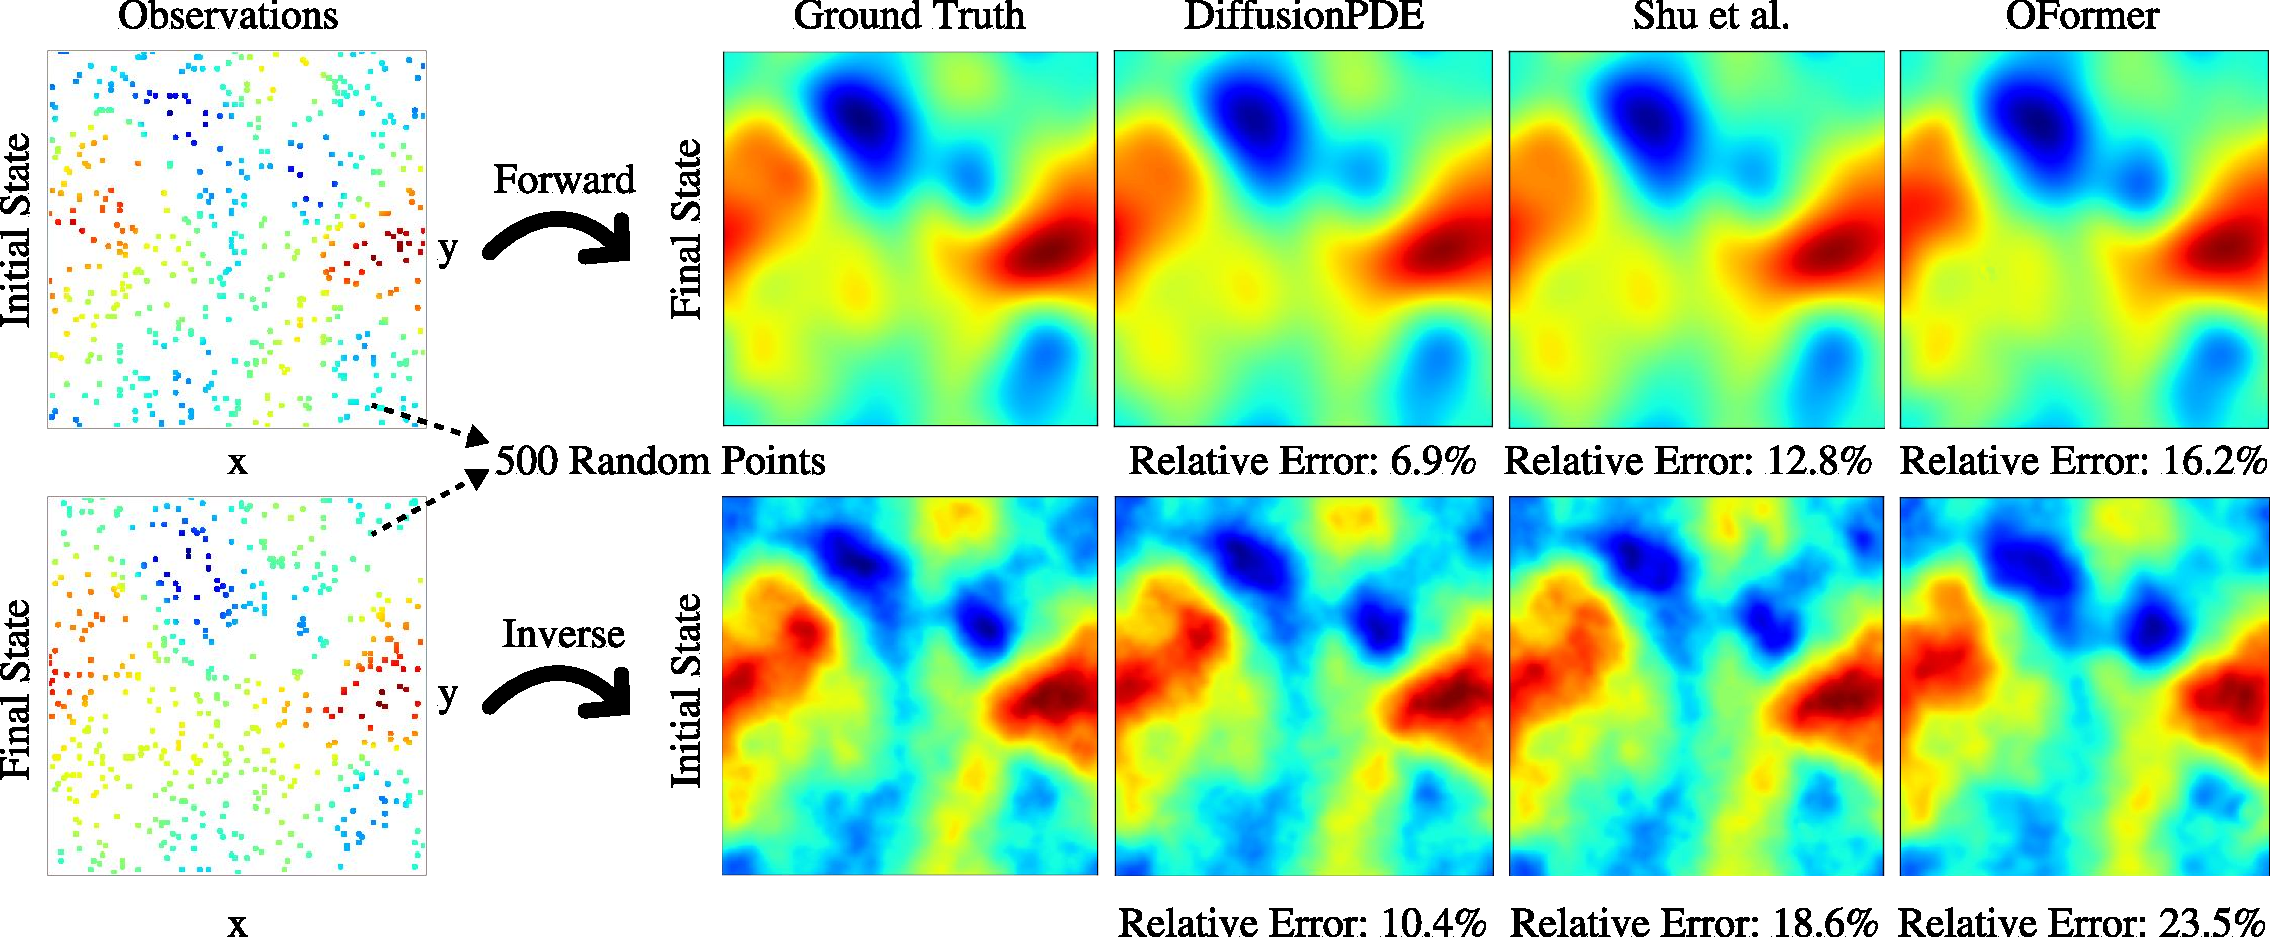
\includegraphics[width=0.8\textwidth]{figs/rebuttal/DiffusionPDE_38.pdf}
    \caption{We compare our DiffusionPDE method with the approaches of Shu et al. \cite{shu2023physics} and OFormer \cite{li2022transformer} for the unbounded Navier-Stokes equation. Using 500 observation points, DiffusionPDE effectively solves both the forward and inverse problems, achieving significantly lower errors.}
    \label{fig:vs-shu-and-oformer}
\end{figure}
